% Set the path for the figures of this chapter
\graphicspath{{Chap1/figures/}}

% Try to have all specifal definition the ../main.tex file. Here just name definitions that are used in a different way in another chapter.
\setlength{\tabcolsep}{12pt}

\chapter[Short chapter title for header and toc]{Long chapter title\footnote{
This chapter is joint work with A, B, and C. This chapter is reprinted with minor edits from Ref.~X.
}}\label{chap:impact_of_technologies}
\begin{chapterabstract}
    How to write an abstract:\footnote{
		Copied from \cite{boyce2010global} with comments and a note form \textit{Nature Education}:
		With just under 200 words, this abstract can convey the motivation for and outcome of the work with some accuracy, without intimidating readers by its length.
		If the journal allows to have the abstract as multiple paragraphs, start a new one before the findings.
	}
	\textbf{(Context)} In the oceans, ubiquitous microscopic phototrophs (phytolankton) account for approximately half the production of organic matter on Earth, thus affecting the abundance and diversity of marine organisms and strongly influencing
	climate processes.
	\textbf{(What we have)} Analyses of the satellite-derived phytoplankton concentration (available since 1979) have suggested decadal fluctuations linked to climate forcing, but the length of this record is insufficient to resolve longer-term trends.
	\textbf{(What we want)} To estimate the time dependence of phytoplankton biomass since the beginning of oceanographic measurements in 1899, 
	\textbf{(Task)}	we combined available ocean transparency measurements and in situ chlorophyll observations.
	\textbf{(Object of the document)} This paper presents the trends we identified at local, regional, and global scales.
	\textbf{(Findings)} We observed declines in eight out of ten ocean regions, and estimated a global rate of decline of $\sim 1\%$ of the global median
	per year. Our analyses further revealed interannual to decadal phytoplankton fluctuations superimposed on long-term trends.
	These fluctuations are strongly correlated with basin-scale climate indices, whereas the long-term declining trends are	related to increasing sea surface temperatures.
	\textbf{(Conclusion)} In conclusion, global phytoplankton concentration has definitely declined over the past century; 
	\textbf{(Perspectives)} this decline will need to be considered	in future studies of marine ecosystems, geochemical cycling,
	ocean circulation, and fisheries.
\end{chapterabstract}

\maketitle

\section{Introduction}
%
Lorem ipsum dolor sit amet, consectetur adipiscing elit. Sed dignissim blandit vestibulum. Etiam feugiat lorem ipsum, non rhoncus tortor pretium eu. Aenean hendrerit metus id sem gravida, id pulvinar nunc gravida. In bibendum blandit ligula quis tempus. Aenean vel congue nulla. Maecenas tempus iaculis arcu. Pellentesque dictum, tortor at commodo semper, risus erat tempus urna, ut scelerisque lacus metus mattis lorem. Sed accumsan dolor at hendrerit pellentesque. Mauris at maximus turpis. Vestibulum convallis cursus euismod. Suspendisse erat metus, pretium id auctor eleifend, vestibulum nec lectus. Donec elementum diam in imperdiet euismod. Nullam molestie consectetur velit, et ullamcorper nisi pharetra vel. Nulla odio mauris, varius a tempus ac, fermentum non enim.

Nulla vulputate hendrerit accumsan. Cras tincidunt tellus imperdiet, fermentum libero ac, ullamcorper odio. Maecenas eu viverra neque. Suspendisse iaculis vulputate turpis, eu convallis leo ullamcorper ut. Proin faucibus mauris eget elementum venenatis. Interdum et malesuada fames ac ante ipsum primis in faucibus. Vestibulum posuere leo sed est ultricies rutrum.

Curabitur malesuada sem a vestibulum vehicula. In condimentum posuere pretium. Etiam tempus gravida sem at fringilla. Praesent luctus sodales tempor. Aliquam erat volutpat. Ut sed metus at purus sollicitudin rutrum. Nulla ullamcorper, nibh in pretium consectetur, ex felis bibendum dui, vitae fringilla magna diam quis ante. Suspendisse fringilla neque in orci tempor laoreet. Fusce vestibulum felis ante, eget tempor nulla lobortis eget. Sed id fringilla neque. Maecenas ullamcorper sit amet neque et fringilla. Mauris convallis enim sapien, id ultrices justo sodales sed. Etiam sagittis arcu quam, non posuere justo eleifend eu.

\section{Methods}\label{sec:methods}

\begin{figure}
	\centering
	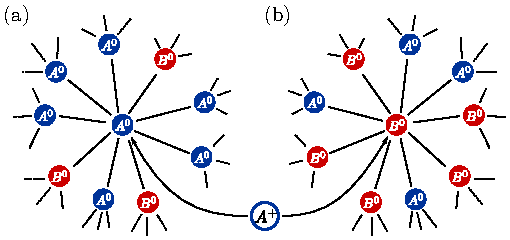
\includegraphics[scale = 1]{technology_draft}
	\caption{\textbf{Caption title.}
		Caption text body.
	}
	\label{fig:technology_draft}
\end{figure}
Text body to discuss \figref{fig:technology_draft}.


\section{Results}\label{sec:results}
Text body.

\section{Discussion} \label{sec:discussion}
Text body.

\begin{subappendices}
\section{Appendix chapter related to this chapter} \label{app:chapter_01}
Text body.
\end{subappendices}
